% ----------------------------------------------------------------
% AMS-LaTeX Paper ************************************************
% **** -----------------------------------------------------------
\documentclass[10pt]{amsart}
%\textwidth 14.5cm
%\textheight 22cm
%\hoffset -1.5cm
%\voffset -2.2cm
\usepackage{graphicx}
\usepackage{latexsym}
\usepackage{amsfonts}
\usepackage{amsthm}
\usepackage{amssymb}
\usepackage{amsmath}
\usepackage{enumerate}
\usepackage{color}
\usepackage{stmaryrd}
\usepackage{chemarrow}
\usepackage[all]{xy}
\usepackage[pdftex,bookmarksnumbered,bookmarksopen,colorlinks,linkcolor=blue,anchorcolor=black,citecolor=blue,urlcolor=blue]{hyperref}
\usepackage{booktabs}
\usepackage{makecell}
\usepackage{subfigure}

%\usepackage{mathabx}
% ----------------------------------------------------------------
\vfuzz2pt % Don't report over-full v-boxes if over-edge is small
\hfuzz2pt % Don't report over-full h-boxes if over-edge is small
% THEOREMS -------------------------------------------------------
\newtheorem{thm}{Theorem}[section]
\newtheorem{cor}[thm]{Corollary}
\newtheorem{lem}[thm]{Lemma}
\newtheorem{prop}[thm]{Proposition}
\theoremstyle{definition}
\newtheorem{defn}[thm]{Definition}
\theoremstyle{remark}
\newtheorem{rem}[thm]{Remark}
%\numberwithin{equation}{section}
% MATH -----------------------------------------------------------
\newcommand{\norm}[1]{\left\Vert#1\right\Vert}
\newcommand{\abs}[1]{\left\vert#1\right\vert}
\newcommand{\set}[1]{\left\{#1\right\}}
\newcommand{\Real}{\mathbb R}
\newcommand{\eps}{\varepsilon}
\newcommand{\To}{\longrightarrow}
\newcommand{\BX}{\mathbf{B}(X)}
\newcommand{\A}{\mathcal{A}}

\newcommand{\dx}{\,{\rm d}x}
\newcommand{\dd}{\,{\rm d}}
\newcommand{\bs}{\boldsymbol}
\newcommand{\mcal}{\mathcal}

\DeclareMathOperator*{\img}{img}
%\DeclareMathOperator*{\span}{span}
\newcommand{\sign}{\operatorname{sign}}
\newcommand{\curl}{\operatorname{curl}}
\renewcommand{\div}{\operatorname{div}}
%\renewcommand{\grad}{\operatorname{grad}}
\newcommand{\grad}{\operatorname{grad}}
\newcommand{\tr}{\operatorname{tr}}
% \DeclareMathOperator*{\tr}{tr}
\DeclareMathOperator*{\rot}{rot}
\DeclareMathOperator*{\var}{Var}
\newcommand{\dev}{\operatorname{dev}}
\newcommand{\sym}{\operatorname{sym}}
\newcommand{\skw}{\operatorname{skw}}
\newcommand{\spn}{\operatorname{spn}}
\newcommand{\mspn}{\operatorname{mspn}}
\newcommand{\mskw}{\operatorname{mskw}}
\newcommand{\vskw}{\operatorname{vskw}}
\newcommand{\vspn}{\operatorname{vspn}}
\newcommand{\defm}{\operatorname{def}}
\newcommand{\hess}{\operatorname{hess}}
% ----------------------------------------------------------------
\begin{document}

\title{\large Detailed Response to Referees}%

\date{}%
%\dedicatory{}%
%\commby{}%
% ----------------------------------------------------------------

\maketitle

For the convenience of narration, we abbreviate standard conforming virtual emelemt
method as CVEM, standard non-conforming virtual emelemt method as NCVEM, 
stabilization-free conforming virtual element method as SFCVEM
and stabilization-free non-conforming virtual element method as SFNCVEM,
In addition, all experiments in this paper were conducted on a PC with AMD Ryzen
5 3500U CPU and 64-bit Ubuntu 22.04 operating system.

\begin{enumerate}[1.]

\item \textsf{
in the numerical section; I agree that it is important to check the rate of
convergence of the method;}

\textsf{However, the convergence does not automatically
guarantee the invertibility of the local stiffness matrices, as imposing the
Dirichlet boundary conditions may have a “stabilizing effect”. So, you should
investigate the number of zero eigenvalues of the local stiffness matrix.}

\textsf{For instance, pick three different hexagonal elements with a fixed degree of
accuracy, e.g., k = 3: the first being a regular hexagon; the second being a
quasi-regular hexagon (small perturbation of the previous element); the third
being a square with an edge containing two hanging nodes. Check whether the
stiffness matrix always has only one zero eigenvalue, i.e., the method is indeed
stabilization free; 
}

\smallskip \noindent \textcolor[rgb]{1.00,0.00,0.00}{Reply.}
\begin{figure}[h]
\centering
\subfigure{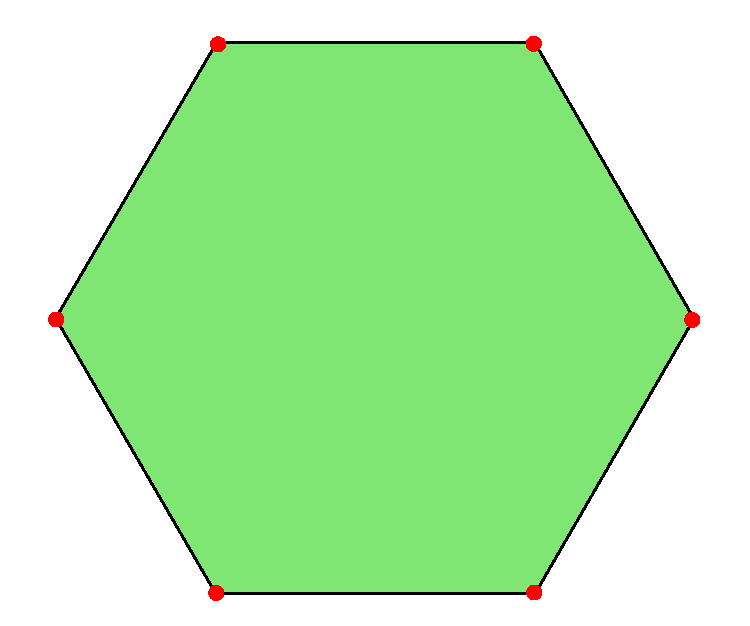
\includegraphics[width=1.4in]{../figures/hexagon0.pdf}}
    % \caption{Type I:5 tetrahedra}
%%
\subfigure{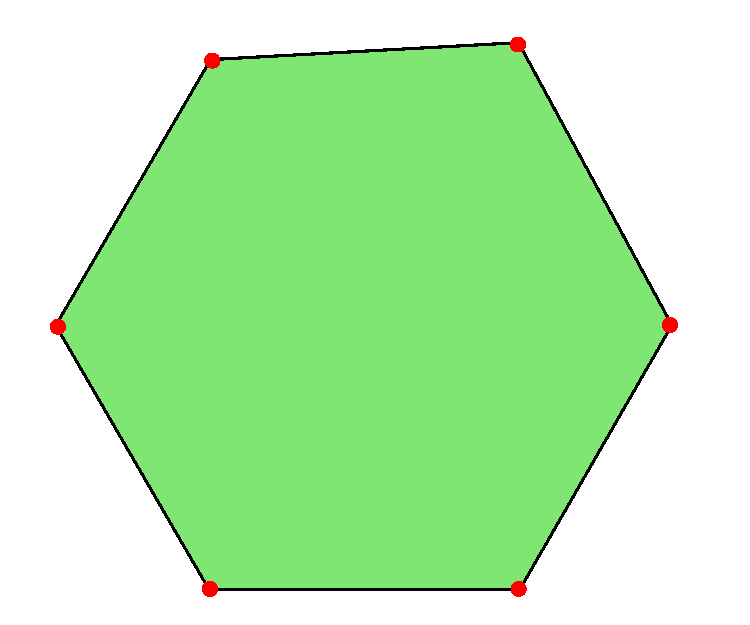
\includegraphics[width=1.4in]{../figures/hexagon1.pdf}}
     %\caption{Type II: 24 tetrahedra}
%%
\subfigure{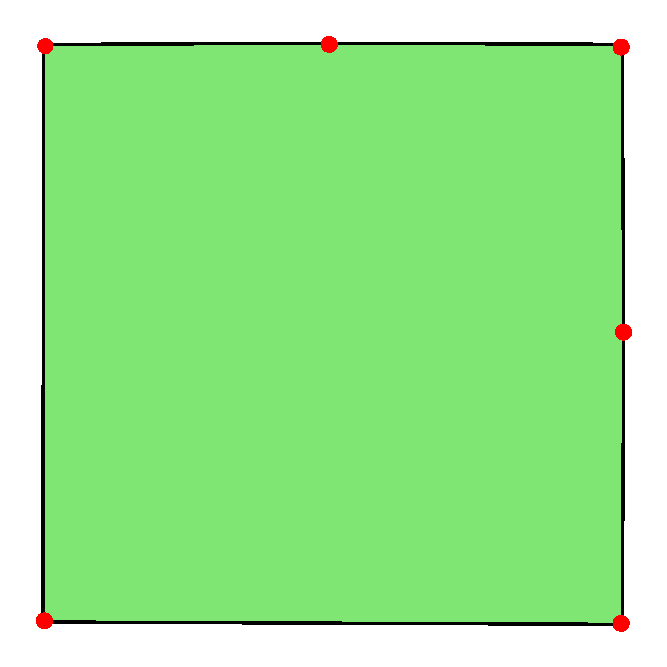
\includegraphics[width=1.2in]{../figures/hexagon2.pdf}}
     %\caption{Trirectangular tetrahedron}
%%
\caption{The regular hexagon(Left), the quasi-regular hexagon generated by regular
    hexagon with a small perturbation (Middle), 
and the square with two hanging nodes (Right)}
  \label{fig:hexagon} %% label for entire figure
\end{figure}

We constructed three different hexagonal elements, 
shown in Figure \ref{fig:hexagon}, and calculated the eigenvalues of local stiffness
matrices with $k=3$. Our numerical results show that, on each element, the number of zero
eigenvalues is only one, indicating that the method is stabilization-free. The
minimum non-zero eigenvalue and the maximum eigenvalue for each element are
shown in Table \ref{tab:comparison0}-\ref{tab:comparison2}:

\begin{table}[h]
\centering
\caption{Comparison of Eigenvalues and Condition Numbers on regular hexagon.}
\label{tab:comparison0}
\begin{tabular}{c|ccc}
\toprule
\textbf{Method} & \textbf{Maximum Eigenvalue} & \textbf{Minimum Nonzero
Eigenvalue} & \textbf{Condition Number} \\ \hline
NCVEM & 975.5693189 & 0.309674737 & 3150.303211 \\ \hline
CVEM & 1012.488116 & 0.297206358 & 3406.683909 \\ \hline
SFNCVEM & 992.5956147 & 0.318932029 & 3112.248147 \\ \hline
SFCVEM & 1011.173331 & 0.298509692 & 3387.405362 \\
\bottomrule
\end{tabular}
\end{table}

\begin{table}[h]
\centering
\caption{Comparison of Eigenvalues and Condition Numbers of quasi-regular hexagon}
\label{tab:comparison1}
\begin{tabular}{c|ccc}
\toprule
\textbf{Method} & \textbf{Maximum Eigenvalue} & \textbf{Minimum Nonzero
Eigenvalue} & \textbf{Condition Number} \\ \hline
NCVEM   & 935.2883848 & 0.279027715 & 3351.955143 \\ \hline
CVEM    & 1014.672395 & 0.257370621 & 3942.456177 \\ \hline
SFNCVEM & 997.4831245 & 0.282126359 & 3535.589964 \\ \hline
SFCVEM  & 1047.876056 & 0.258970708 &
4046.311124 \\
\bottomrule
\end{tabular}
\end{table}

\begin{table}[h]
\centering
\caption{Comparison of Eigenvalues and Condition Numbers of quasi-regular hexagon}
\label{tab:comparison2}
\begin{tabular}{c|ccc}
\toprule
\textbf{Method} & \textbf{Maximum Eigenvalue} & \textbf{Minimum Nonzero
Eigenvalue} & \textbf{Condition Number} \\ \hline
 NCVEM   & 941.8571938&	0.21069027	&4470.340249 \\ \hline
 CVEM    & 1046.755495&	0.200435123	&5222.4155 \\ \hline
 SFNCVEM & 986.5963357&	0.212761106	&4637.108513 \\ \hline
 SFCVEM  & 1061.651989&	0.202074633	&5253.761808 \\
\bottomrule
\end{tabular}
\end{table}


\item \textsf{
my feeling is that the proposed stabilization-free approach is much more
expensive than the standard one. Thus, you should check the assembling time
of the stabilization-free and standard VEMs, on: (i) a (reasonably large)
sequence of meshes; (ii) fixing a mesh, increasing the degree of accuracy,
e.g., up to $k = 10$.
}
\begin{figure}[h]
\centering
\subfigure{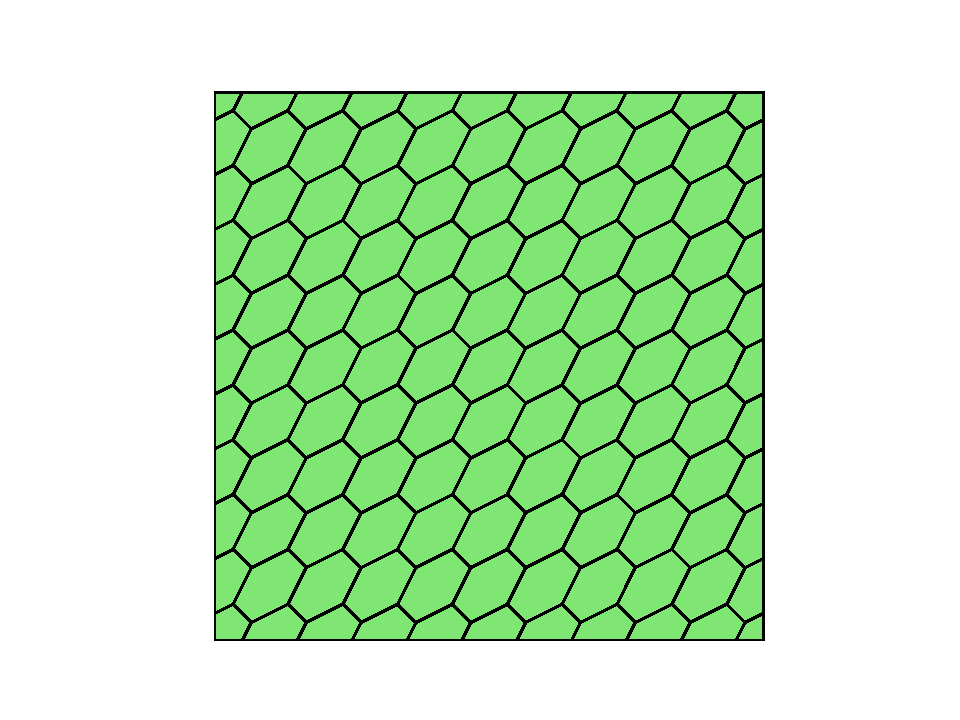
\includegraphics[width=2.2in]{../figures/poly_mesh.pdf}}
\subfigure{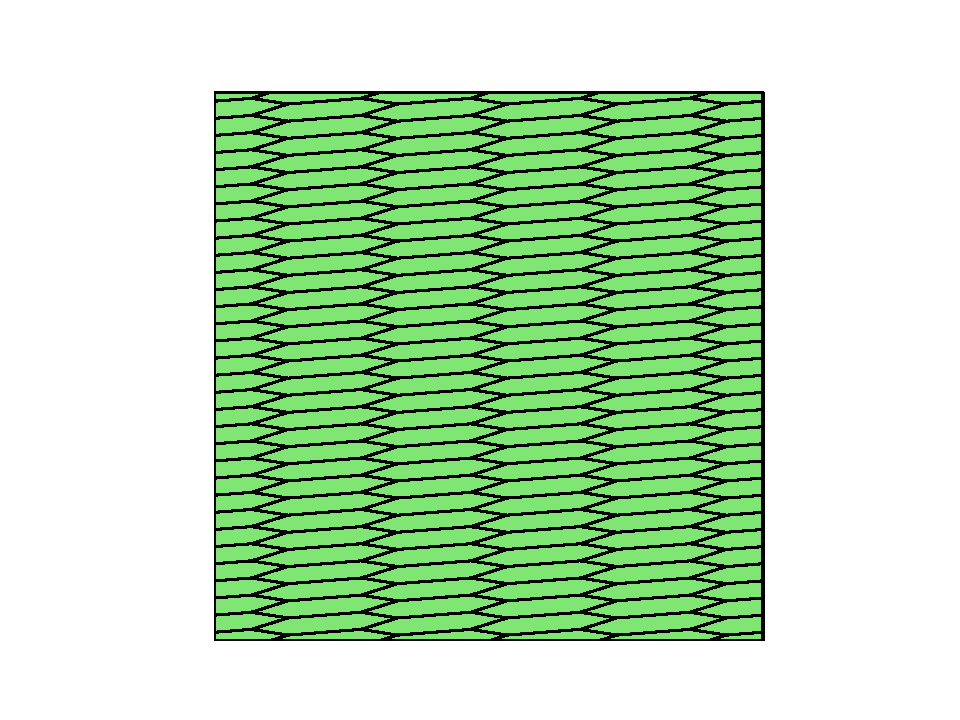
\includegraphics[width=2.2in]{../figures/mesh_hy.pdf}}
\caption{The mesh of domain $(0, 1)\times(0, 1)$. Left: $h = 0.1$. Right:
$h_x=0.2, h_y = 0.03125$.}
  \label{fig:polymesh} %% label for entire figure
\end{figure}

\smallskip \noindent \textcolor[rgb]{1.00,0.00,0.00}{Reply.}
The only difference between standard method and stabilization-free method is the
assembly of stiffness matrix,
so we compared in detail the time to assemble the stiffness matrix with
different methods when changing degree of accuracy $k$ and mesh size $h$
respectively. Figure \ref{fig:polymesh} depicts the mesh used to partition domain 
$(0, 1)\times(0, 1)$ with mesh size for this experiment.
The results presented in Table
\ref{tab:ptime}, \ref{tab:ttime}, that
NCVEM, CVEM, SFNCVEM have similar assembling times. 
However, SFCVEM requires additional time due to the projection to a higher
degree of polynomial space.

\begin{table}[htbp]
\caption{Comparison of four methods in assembling stiffness matrix time with
 $h=0.2$, $k = \{2, 4, 8, 10\}$.}
\label{tab:ptime}
\centering
\begin{tabular}{c|cccc}
\toprule
$k$ & 2 & 4 & 8 & 10 \\
\hline
SFCVEM & 0.053684235 & 0.144996881 & 1.468627453 & 2.603836536 \\
SFNCVEM & 0.022516727 & 0.065697193 & 0.806378841 & 1.554260015 \\
CVEM & 0.021185875 & 0.059809923 & 0.600241184 & 1.160929918 \\
NCVEM & 0.0213027 & 0.061014891 & 0.596506596 & 1.129639149 \\
\bottomrule
\end{tabular}
\end{table}

\begin{table}[htbp]
\caption{Comparison of four methods in assembling stiffness matrix time with
 $h=\{1, 0.25, 0.0625, 0.03125\}$, $k = 5$.}
\label{tab:ttime}
\begin{tabular}{c|cccc}
\toprule
$h$ &    1	& 0.25 & 0.0625 & 0.03125\\
\hline
SFCVEM & 0.039689541 & 0.199015379	& 1.74412179	& 4.75462532\\
SFNCVEM & 0.018287182 & 0.100006819	& 0.81251812	& 2.465409517\\
CVEM & 0.018686771 & 0.087426662	& 0.781031132	& 1.983617783\\
NCVEM & 0.018309593 & 0.096345425	& 0.767129898	& 2.159288645\\
\bottomrule
\end{tabular}
\end{table}

\begin{figure}[h]
\centering
\subfigure{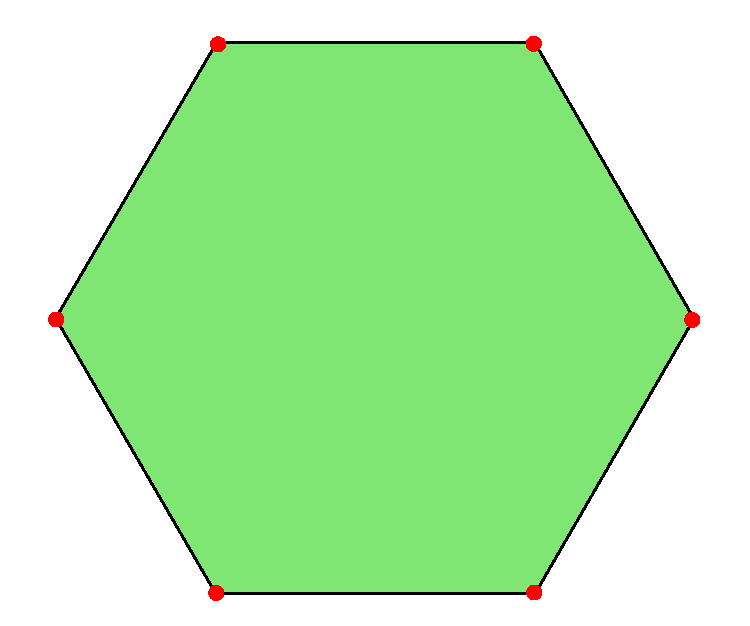
\includegraphics[width=1.4in]{../figures/hexagon0.pdf}}
    % \caption{Type I:5 tetrahedra}
%%
\subfigure{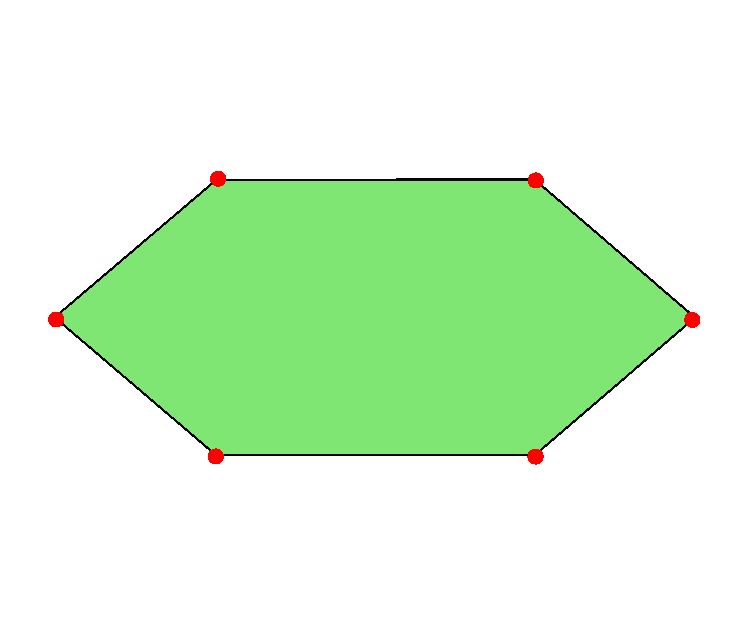
\includegraphics[width=1.4in]{../figures/hexagon3.pdf}}
     %\caption{Type II: 24 tetrahedra}
%%
\subfigure{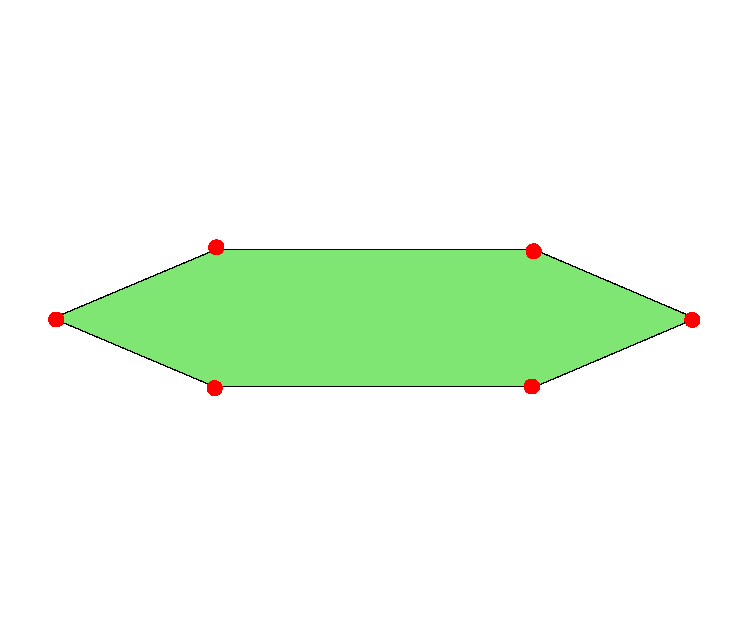
\includegraphics[width=1.4in]{../figures/hexagon4.pdf}}
     %\caption{Trirectangular tetrahedron}
%%
\caption{The hexagon $H_0, H_1, H_2$.}
  \label{fig:collapsehexagon} %% label for entire figure
\end{figure} 

\item \textsf{
along the same avenue, you should also compare the condition number of the
global matrices obtained with the two approaches in the two situations (i) and
(ii) above. Furthermore, you may also wish to consider sequences of meshes with
“collapsing elements” (refine a mesh and change the aspect ratio), and check the
condition numbers again.  As a suggestion, since the condition number should be
computed scaling the diagonal of the matrix, you can empirically check such
conditioning by testing the two approaches on a patch test. The conditioning can
be estimated checking the growth of the error for the patch test.
}

\smallskip \noindent \textcolor[rgb]{1.00,0.00,0.00}{Reply.}
We designed two experiments to check the condition number of the stiffness
matrix. Firstly, we refer to the ``collapsing polygons'' experiment in
\cite{Mascotto2018} and consider a hexagonal sequence
$\{H_i\}_{i=0}^{\infty}$, where the vertices of $H_i$ are as follows:

$$
A_i = (1, 0), B_i = (0.5, a_i), C_i = (-0.5, a), D_i=(-1, 0), 
$$
$$
E_i = (-0.5, -a_i), F_i = (0.5, -a_i)
$$
where $a_i = \frac{\sqrt{3}}{2^{i+1}}$, the image of $\{H_0, H_1, H_2\}$ shown
in Figure \ref{fig:collapsehexagon}. 

We construct the virtual element space on $H_i$ and calculate the condition number
of the stiffness matrix of four methods. As shown in Figure
\ref{fig:collapsehexagon_conditionnumber}, the condition numbers of stiffness
matrix obtained by stabilization-free method are smaller than obtained by
standard method when $i$ is large.

\begin{figure}[h]
\centering
\subfigure{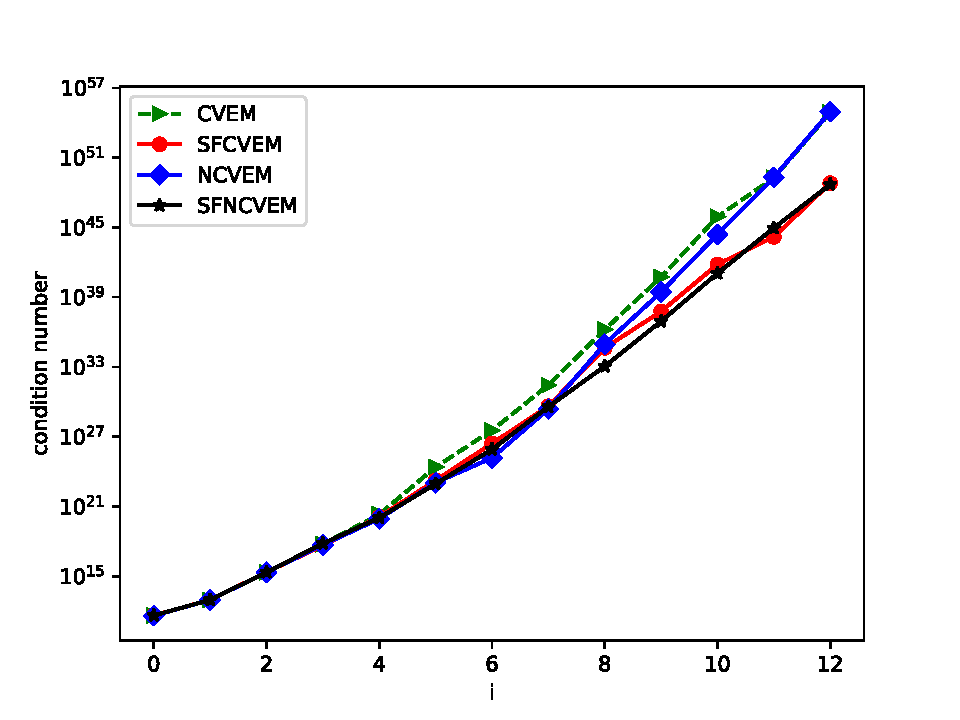
\includegraphics[width=2.2in]{../figures/collapsing_condition_number_8.pdf}}
\subfigure{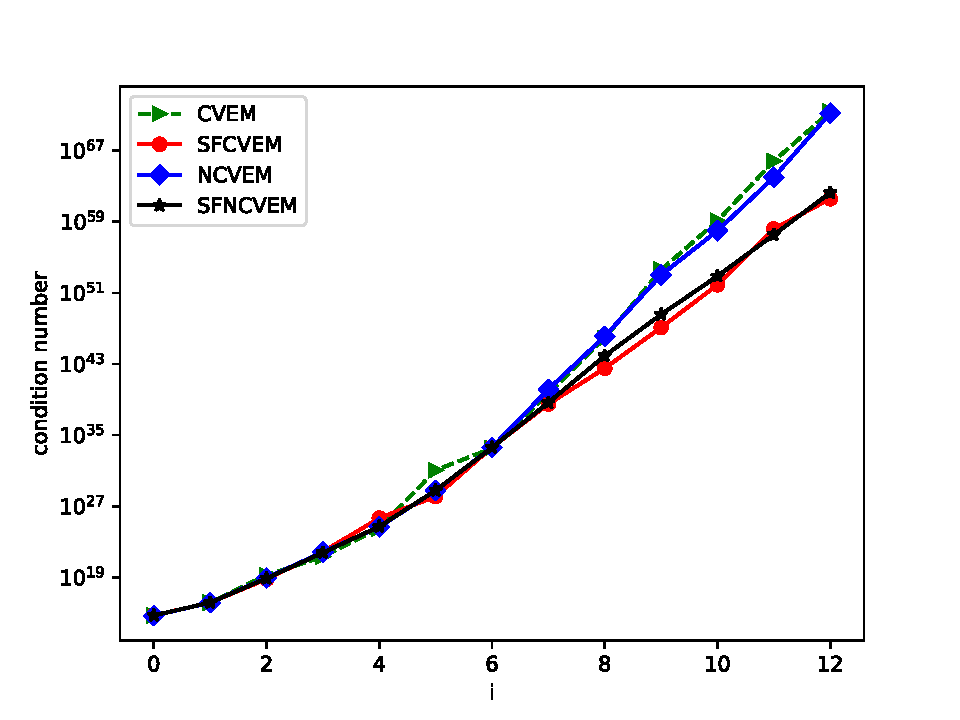
\includegraphics[width=2.2in]{../figures/collapsing_condition_number_10.pdf}}
\caption{The condition number of stiffness matrix four method on
$\{H_i\}_{i=0}^{12}$, Left : $k = 8$, Right : $k = 10$.}
  \label{fig:collapsehexagon_conditionnumber} %% label for entire figure
\end{figure}

Secondly,  consider the patch test problems:

$$
\left\{\begin{aligned}
-\Delta u & = 0 \quad x \in \Omega\\
u & = g \quad x \in \partial \Omega
\end{aligned}\right.
$$

where $\Omega = (0, 1)^2, \ u = g = 1+x+y$. 

Set $h_x$ is size of mesh in the x-direction, $h_y$ is size of mesh in the
y-direction,
we computed the numerical solution $u_h$ of patch test by four methods, and
observe the behavior of $L^2$ errors $||u - u_h||_0$ of patch test in the
following three ways:
\begin{enumerate}[(1)]
\item Fix $h_x=h_y=0.2$, change $k= 1, 2, 3, 4, 5, 6, 7, 8, 9, 10$.
\item Fix $k=3$, change $h_x=h_y=\frac{1}{2}, \frac{1}{4}, \frac{1}{8},
     \frac{1}{16}, \frac{1}{32}$.
\item Fix $k=3$, $h_x=0.2$, change $h_y=\frac{1}{2}, \frac{1}{4}, \frac{1}{8},
    \frac{1}{16}, \frac{1}{32}, \frac{1}{64}, \frac{1}{128}, \frac{1}{256}$.
\end{enumerate}

The errors are shown in Figure \ref{fig:patchtest}, where 
the errors of four methods are similar. 
Furthermore, 
the condition numbers of the stiffness matrix obtained by
four methods are similar, because of the error in the patch test is to
grow as the condition number of the stiffness matrix grows
\cite{DassiMascotto2018}.

\begin{figure}[h]
\centering
\subfigure{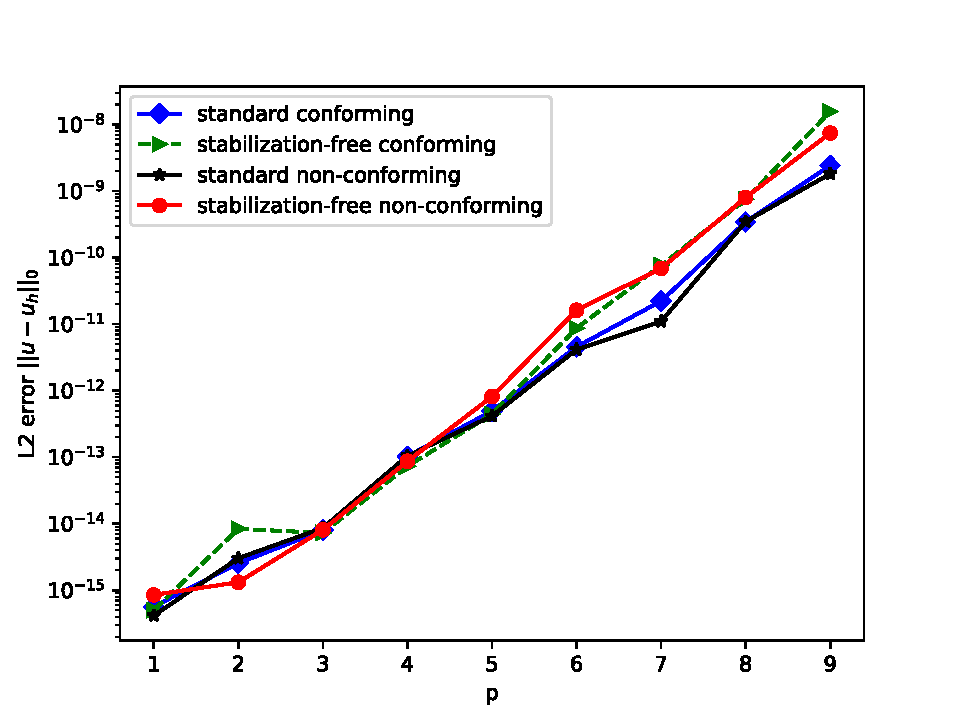
\includegraphics[width=2.2in]{../figures/patch_test_p.pdf}}
    % \caption{Type I:5 tetrahedra}
%%
\subfigure{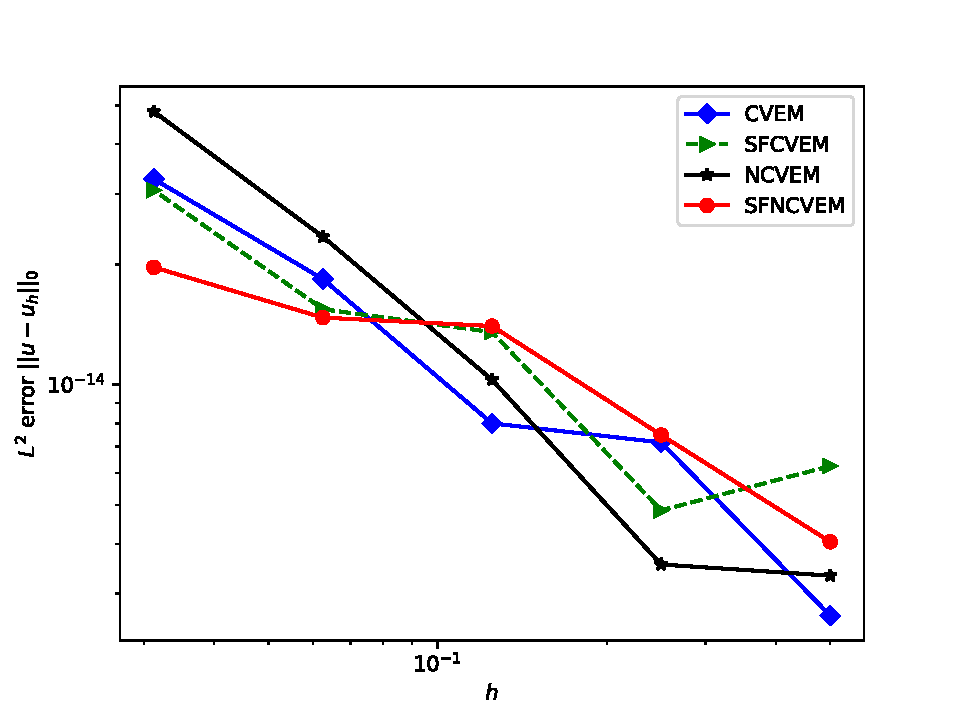
\includegraphics[width=2.2in]{../figures/patch_test_h.pdf}}
     %\caption{Type II: 24 tetrahedra}
%%
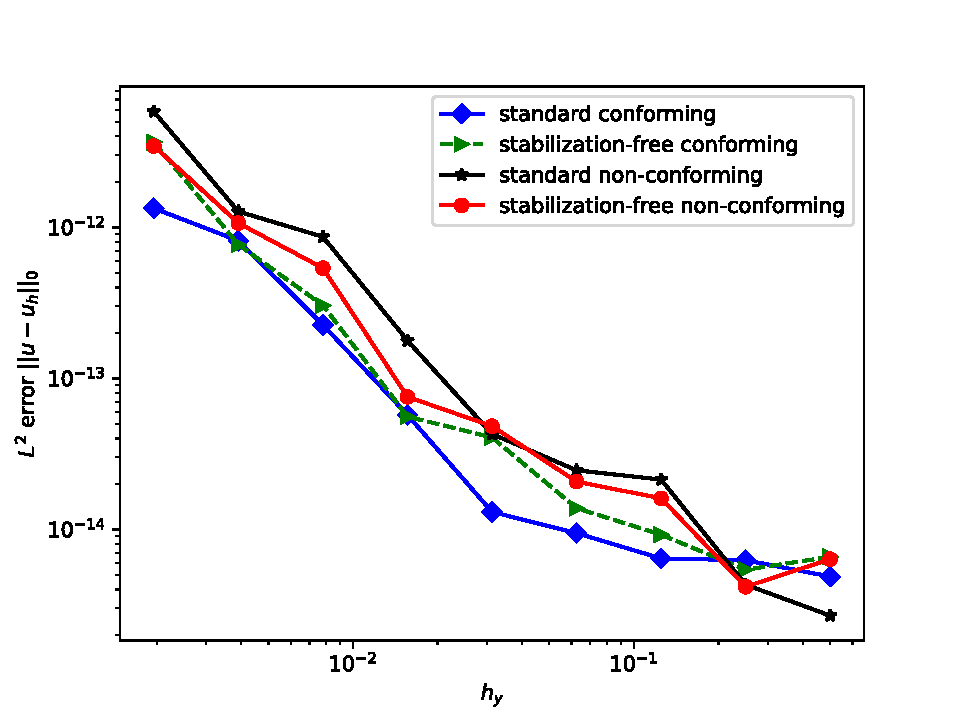
\includegraphics[width=2.2in]{../figures/patch_test_hy.pdf}
  \label{fig:patchtest} %% label for entire figure
\caption{The $L^2$ error of patch test.}
\end{figure}

















 
\end{enumerate}

\end{document}
